\documentclass[11pt,a4paper]{article}

\usepackage[spanish]{babel}
\usepackage[utf8]{inputenc}
\usepackage[T1]{fontenc}
\usepackage[margin=2.5cm]{geometry}
\usepackage{amsmath,amssymb}
\usepackage{booktabs}
\usepackage{siunitx}
\usepackage{graphicx}
\usepackage{tikz}
\usetikzlibrary{arrows.meta,positioning,shapes.geometric}
\usepackage{caption}
\usepackage[colorlinks=true,linkcolor=blue!50!black,citecolor=blue!50!black,urlcolor=blue!50!black]{hyperref}
\usepackage[backend=biber,style=ieee,sorting=none]{biblatex}
\addbibresource{references.bib}

\sisetup{output-decimal-marker={,}, group-separator={\,}}

\newcommand{\repoteam}{\url{https://github.com/carlospatroner-boop/pe-u4-spark-Soporte-Tecnico-ISP}}
\newcommand{\committeam}{\texttt{d9ce0e69ab81c4a8b7373c5a29f0522dc048f2f9}}

\title{}
\date{}

\begin{document}

% ============================================================
% PORTADA
% ============================================================
\begin{titlepage}
\centering
{\large\bfseries UNIVERSIDAD T\'ECNICA ESTATAL DE QUEVEDO\par}
\vspace{0.2cm}
{\normalsize Facultad de Ciencias de la Computaci\'on\par}
{\normalsize Carrera de Ingenier\'ia de Software\par}
\vspace{1.2cm}
\rule{0.8\textwidth}{0.4pt}\par
\vspace{0.6cm}
{\Large\bfseries TA-IND-04 --- Informe T\'ecnico Individual\par}
\vspace{0.3cm}
{\large An\'alisis de Rendimiento Paralelo (Unidad 4) aplicado al Proyecto Fin de Curso\par}
\vspace{0.3cm}
{\normalsize Transformaci\'on individual declarada como foco: \textbf{T1 --- Filtrado y selecci\'on}\par}
\vspace{0.6cm}
\rule{0.8\textwidth}{0.4pt}\par
\vspace{1.0cm}

\begin{tabular}{ll}
\textbf{Asignatura:} & Aplicaciones Distribuidas (ISR-701) \\
\textbf{Unidad:} & Unidad 4 --- C\'omputo Paralelo y Distribuido \\
\textbf{Estudiante:} & Jeremy Alexis Alvarez Parraga \\
\textbf{Correo institucional:} & jalvarezp3@uteq.edu.ec \\
\textbf{Equipo PE-U4 / GA-SUM-05:} & ACC --- Soporte T\'ecnico ISP \\
\textbf{Integrantes del equipo:} & Alvarez Parraga Jeremy Alexis \\
 & Aucatoma Celorio Jhinson Stalyn \\
 & Carpio Mendoza Carlos Jose \\
\textbf{PFC de referencia:} & ACC --- Soporte T\'ecnico ISP (gesti\'on de tickets) \\
\textbf{Docente responsable:} & Gleiston C. Guerrero-Ulloa, M.Sc. \\
\textbf{Per\'iodo acad\'emico:} & 2026--2027 PPA \\
\textbf{Fecha:} & 8 de agosto de 2026 \\
\end{tabular}

\vspace{1.2cm}
\textbf{URL del repositorio individual de entrega (TA-IND-04):}\par
\vspace{0.2cm}
\url{https://github.com/DeJere/TA-IND-04-An-lisis-de-Rendimiento-Paralelo}\par
\textit{\small (Repositorio individual p\'ublico de entrega; ver README.md de este mismo repositorio para la lista de verificaci\'on previa a la entrega.)}

\vspace{1.2cm}
\textbf{Repositorio de origen de los datos (equipo PE-U4, sin modificaciones):}\par
\vspace{0.2cm}
\repoteam\par
\textbf{Commit declarado:} \committeam

\end{titlepage}

% ============================================================
\section{Introducci\'on y contexto}
% ============================================================

Este informe desarrolla el objetivo de TA-IND-04: analizar cr\'iticamente, de forma
individual, los resultados de \textit{speedup} obtenidos por el equipo ACC en la pr\'actica
PE-U4/GA-SUM-05 (comprobaci\'on experimental de la Ley de Amdahl con Apache Spark), y a
partir de ese diagn\'ostico fundamentar una propuesta de integraci\'on del procesamiento
distribuido en el Proyecto Fin de Curso (PFC) declarado por el equipo: \textit{ACC ---
Soporte T\'ecnico ISP}, un sistema de gesti\'on de tickets de soporte t\'ecnico para un
proveedor de servicios de internet.

El experimento de PE-U4 compar\'o cinco transformaciones (T1--T5) implementadas en dos
motores --- pandas (secuencial, un solo hilo efectivo) y PySpark (distribuido) --- sobre un
extracto de \num{600000} tickets reales de quejas de consumidores contra proveedores de
telecomunicaciones, publicado por la \textit{Federal Communications Commission} (FCC) de
EE.\,UU. bajo dominio p\'ublico~\cite{fccdataset2026}. Cada transformaci\'on se midi\'o con
el protocolo com\'un del equipo (\texttt{src/\allowbreak{}medicion.py}): una repetici\'on de calentamiento
descartada y cinco repeticiones cronometradas con \texttt{time.perf\_counter()}, reportando
la mediana; para PySpark, cada repetici\'on fuerza la materializaci\'on del resultado con
\texttt{count()} antes de detener el cron\'ometro.

Como transformaci\'on individual de foco se declara \textbf{T1 --- Filtrado y selecci\'on}
(\texttt{src/\allowbreak{}transformaciones\_spark.py::\allowbreak{}t1\_filtrado}), que retiene \'unicamente los
tickets de canal \texttt{Phone} o \texttt{Internet} con \texttt{method}, \texttt{city} y
\texttt{state} no nulos, proyectando las columnas
\texttt{id, ticket\_created, issue\_type, method, issue, city, state}. Sobre las
\num{600000} filas de entrada, T1 retiene \num{558289} filas (\num{454665} de tipo
\textit{Phone} y \num{103624} de tipo \textit{Internet}), con equivalencia exacta de
cardinalidad y de distribuci\'on entre pandas y PySpark seg\'un
\texttt{resultados/\allowbreak{}equivalencia.json} del equipo.

\paragraph{Trazabilidad de los datos base.} Todas las cifras num\'ericas de este informe
provienen, sin alteraci\'on, del repositorio p\'ublico del equipo PE-U4 en el commit
declarado en la portada:
\begin{itemize}
  \item \textbf{Repositorio:} \repoteam
  \item \textbf{Commit:} \committeam{} (\texttt{HEAD} de \texttt{main} al momento de la consulta)
  \item \textbf{Archivo de origen de los tiempos:} \texttt{resultados/\allowbreak{}tiempos\_resumen.csv},
    \texttt{resultados/\allowbreak{}tiempos\_crudos.csv}, \texttt{resultados/\allowbreak{}amdahl\_fit.json},
    \texttt{resultados/\allowbreak{}t3\_escalado\_executors.json}, \texttt{resultados/\allowbreak{}equivalencia.json}.
  \item \textbf{Plataforma de ejecuci\'on declarada por el equipo:} contenedor Docker
    (\texttt{eclipse-\allowbreak{}temurin:21-\allowbreak{}jdk-\allowbreak{}jammy}, Java~21) con \textbf{PySpark~4.1.2}, ejecutado
    localmente (\texttt{local[N]}) --- no Google Colab ni Databricks Community Edition, las
    dos plataformas sugeridas a modo de ejemplo en la gu\'ia. Se declara expl\'icitamente
    esta diferencia por transparencia: el equipo document\'o y reprodujo su propio entorno
    v\'ia Docker (\texttt{README.md} del repositorio de origen), lo cual es igualmente
    verificable y no afecta la validez de las cifras.
  \item \textbf{Configuraci\'on efectiva de Spark para T1} (\texttt{resultados/\allowbreak{}spark\_config\_efectiva\_local4.json}):
    \texttt{spark.master=local[4]}, \texttt{spark.executor.\allowbreak{}instances=4},
    \texttt{spark.sql.\allowbreak{}shuffle.\allowbreak{}partitions=8}.
\end{itemize}

No se detect\'o ning\'un error en los datos del equipo que requiriera correcci\'on; las
cifras reportadas en las Secciones~\ref{sec:analisis} y~\ref{sec:diagnostico} son id\'enticas
a las del commit declarado.

% ============================================================
\section{An\'alisis propio de los resultados de \textit{speedup}}
\label{sec:analisis}
% ============================================================

\subsection{Formalizaci\'on}

Con $p$ la fracci\'on paralelizable del algoritmo y $N$ el n\'umero de unidades de
procesamiento, la Ley de Amdahl~\cite{amdahl1967} establece el \textit{speedup} te\'orico y su l\'imite
superior como
\begin{equation}
\begin{aligned}
S(N) &= \frac{1}{(1-p)+\dfrac{p}{N}}, \\[4pt]
S_{\text{m\'ax}} &= \lim_{N\to\infty} S(N) = \frac{1}{1-p}.
\end{aligned}
\label{eq:amdahl}
\end{equation}

La eficiencia del paralelismo se define como
\begin{equation}
E(N) = \frac{S(N)}{N}.
\label{eq:eficiencia}
\end{equation}

El \textit{speedup} observado se calcula directamente como $S = T_{\text{pandas}} /
T_{\text{pyspark}}$, con ambos tiempos expresados en la misma unidad.

\subsection{Tabla de tiempos y \textit{speedup} de las cinco transformaciones}

La Tabla~\ref{tab:tiempos} reproduce, sin alteraci\'on, las medianas de cinco repeticiones
por transformaci\'on (\texttt{resultados/\allowbreak{}tiempos\_resumen.\allowbreak{}csv}, commit \committeam) y agrega
el c\'alculo propio de $S$ y de $E(4)$ mediante la Ec.~\eqref{eq:eficiencia}.

\begin{table}[h]
\centering
\caption{Tiempos base (mediana de 5 repeticiones), \textit{speedup} y eficiencia con $N=4$.
Fuente de $T_{\text{pandas}}$ y $T_{\text{pyspark}}$: \texttt{resultados/\allowbreak{}tiempos\_resumen.\allowbreak{}csv},
commit \committeam. $S$ y $E(4)$ son c\'alculo propio.}
\label{tab:tiempos}
\begin{tabular}{@{}llS[table-format=1.4]S[table-format=1.4]S[table-format=1.4]S[table-format=1.4]@{}}
\toprule
\textbf{Id.} & \textbf{Transformaci\'on} & {$T_{\text{pandas}}$ (s)} & {$T_{\text{pyspark}}$ (s)} & {$S$} & {$E(4)$} \\
\midrule
\textbf{T1} & \textbf{Filtrado y selecci\'on (foco)} & 0.1846 & 1.0789 & \textbf{0.1711} & \textbf{0.0428} \\
T2 & Agrupaci\'on y agregaci\'on & 0.1575 & 1.8854 & 0.0835 & 0.0209 \\
T3 & \textit{Join} de dos \texttt{DataFrames} & 0.1363 & 1.8290 & 0.0745 & 0.0186 \\
T4 & Columna derivada compleja (UDF) & 0.3559 & 0.8483 & 0.4195 & 0.1049 \\
T5 & Ordenamiento y \textit{top-N} & 0.1169 & 1.4286 & 0.0818 & 0.0205 \\
\bottomrule
\end{tabular}
\end{table}

Las cinco transformaciones presentan $S<1$: PySpark, en \texttt{local[4]} sobre
\num{600000} filas, es m\'as lento que pandas en la totalidad de la pr\'actica. Este es el
resultado esperado y documentado por el propio equipo, y constituye el punto de partida del
an\'alisis individual sobre T1.

\subsection{Contraste de T1 frente a la predicci\'on de Amdahl}
\label{sec:contraste-amdahl}

\textbf{Respuesta expl\'icita a la Pregunta 1 (\S\ref{sec:preguntas}): No, el resultado de T1
no coincide con la predicci\'on de Amdahl, y no puede coincidir por construcci\'on
matem\'atica del modelo.} Para $N=4$ y cualquier fracci\'on paralelizable $p\in[0,1]$, la
Ec.~\eqref{eq:amdahl} solo puede tomar valores en el intervalo $S(4)\in[1,4]$: el extremo
inferior $S=1$ corresponde a $p=0$ (algoritmo enteramente secuencial, sin penalizaci\'on ni
beneficio) y el extremo superior $S=4$ a $p=1$ (paralelismo perfecto). El valor medido para
T1, $S_{\text{T1}}=0.1711$, es \textbf{aproximadamente 5,8 veces menor que el m\'inimo
te\'orico alcanzable}, y por lo tanto queda fuera de la regi\'on factible de la Ec.~\eqref{eq:amdahl}
para cualquier valor de $p$. La Figura~\ref{fig:amdahl} ilustra esta brecha: la envolvente de
Amdahl para $N\in[1,8]$ (\'area sombreada, $S\in[1,N]$) nunca desciende de $S=1$, mientras que
el punto medido de T1 cae muy por debajo de esa envolvente completa.

\begin{figure}[h]
\centering
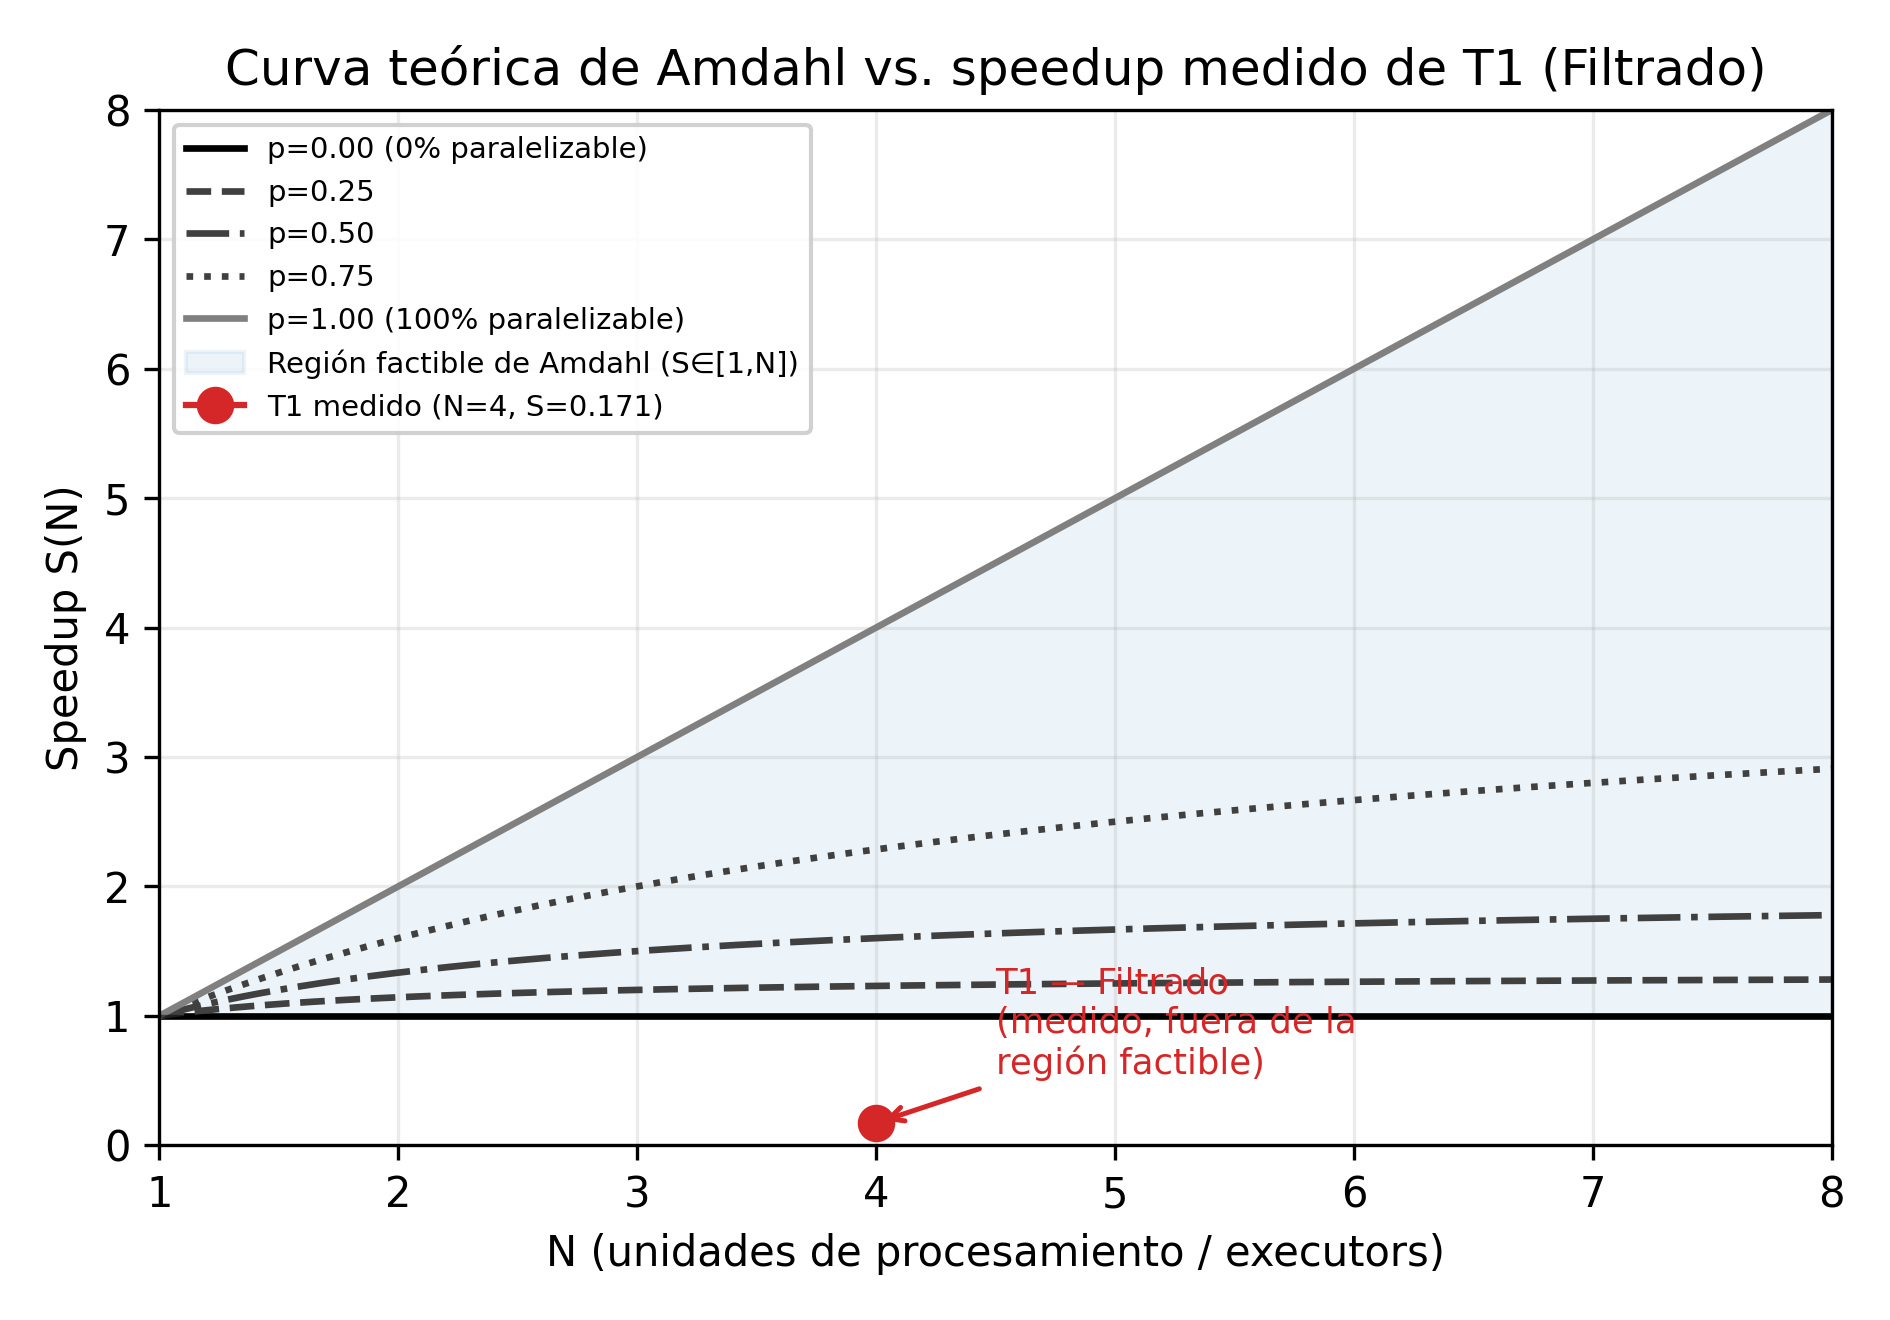
\includegraphics[width=0.72\textwidth]{../figuras/fig_speedup_T1.png}
\caption{Curvas te\'oricas de Amdahl (Ec.~\eqref{eq:amdahl}) para distintos valores de $p$
frente al \textit{speedup} medido de T1 en $N=4$. El \'area sombreada marca la regi\'on
factible $S\in[1,N]$ que el modelo permite para cualquier $p\in[0,1]$; el punto medido de T1
queda muy por debajo de dicha regi\'on. Elaboraci\'on propia (matplotlib, 300\,dpi) a partir de
$S_{\text{T1}}=0{,}1711$ (Tabla~\ref{tab:tiempos}).}
\label{fig:amdahl}
\end{figure}

La \textbf{desviaci\'on relativa} entre el \textit{speedup} medido y el m\'inimo te\'orico
predicho por Amdahl ($S_{\text{teo,m\'in}}=1$, el caso menos favorable del modelo) es
\[
\Delta = \frac{S_{\text{med}} - S_{\text{teo,m\'in}}}{S_{\text{teo,m\'in}}}
       = \frac{0{,}1711 - 1}{1} = -82{,}9\%,
\]
es decir, T1 en PySpark tarda casi 6~veces m\'as que en pandas, cuando el modelo de Amdahl ---
bajo su hip\'otesis de sobrecarga nula por distribuci\'on --- ni siquiera contempla la
posibilidad de que distribuir una tarea la vuelva m\'as lenta que ejecutarla en un solo
proceso. Esto responde exactamente a la tercera respuesta leg\'itima prevista por la gu\'ia
(\textit{speedup} inferior a la unidad): el l\'imite superior que describe la Ec.~\eqref{eq:amdahl}
asume que toda la sobrecarga proviene \'unicamente de la fracci\'on serial $(1-p)$, sin ning\'un
t\'ermino de costo fijo por distribuir el trabajo. Como discuten Hill y Marty al revisar la Ley de Amdahl para la era multin\'ucleo/distribuida~\cite{hillmarty2008}, el modelo cl\'asico no incorpora ning\'un t\'ermino de costo fijo independiente de $p$; un motor real como Spark s\'i incurre en ese
costo fijo (Secci\'on~\ref{sec:diagnostico}), por lo que su tiempo total puede exceder el de la
ejecuci\'on secuencial de referencia, produciendo $S<1$ --- un resultado que la Ec.~\eqref{eq:amdahl}
no puede generar para ning\'un $p$ v\'alido, tal como formaliza el modelo extendido de la
Ec.~\eqref{eq:umbral} en la Secci\'on~\ref{sec:dimensionamiento}.

% ============================================================
\section{Diagn\'ostico de la fracci\'on no escalable y de la sobrecarga}
\label{sec:diagnostico}
% ============================================================

\subsection{M\'etrica de Karp-Flatt}

La fracci\'on serial determinada experimentalmente a partir del \textit{speedup} observado
$S$ con $N$ unidades se calcula, seg\'un Karp y Flatt~\cite{karpflatt1990}, como
\begin{equation}
e = \dfrac{\dfrac{1}{S}-\dfrac{1}{N}}{1-\dfrac{1}{N}}, \qquad N>1.
\label{eq:karpflatt}
\end{equation}

\textbf{Limitaci\'on de datos declarada expl\'icitamente.} T1 se midi\'o, en el protocolo del
equipo, \'unicamente con la configuraci\'on por defecto \texttt{local[4]}
(\texttt{src/\allowbreak{}transformaciones\_spark.\allowbreak{}py:\allowbreak{}:\allowbreak{}medir\_t1\_t2\_t4\_t5}); no existe en el repositorio
declarado ninguna medici\'on de T1 con $N=1$ o $N=2$. La \'unica serie con variaci\'on real de
$N\in\{1,2,4\}$ en todo el repositorio corresponde a T3 (\textit{join}), medida
expresamente para habilitar el an\'alisis de escalabilidad de Amdahl
(\texttt{src/\allowbreak{}transformaciones\_spark.\allowbreak{}py:\allowbreak{}:\allowbreak{}medir\_t3\_escalado},
\texttt{resultados/\allowbreak{}t3\_escalado\_executors.\allowbreak{}json}). Por trazabilidad (Secci\'on~10.2, piso
P4 de la gu\'ia), no se fabrica un punto de T1 en $N=2$: la Ec.~\eqref{eq:karpflatt} se
aplica primero sobre la \'unica serie multi-$N$ real disponible (T3) para cumplir el
requisito de calcular $e$ en $N=2$ y $N=4$, y despu\'es se calcula tambi\'en $e$ para el
\'unico punto real de T1 ($N=4$), interpret\'andolo como diagn\'ostico adicional.

\begin{table}[h]
\centering
\caption{M\'etrica de Karp-Flatt (Ec.~\eqref{eq:karpflatt}) sobre la serie de T3
(\'unica con $N=1,2,4$ trazable en el repositorio, \texttt{resultados/\allowbreak{}amdahl\_fit.\allowbreak{}json}) y
sobre el punto \'unico de T1. $S$ de T3 es relativo a su propio tiempo en $N=1$.}
\label{tab:karpflatt}
\begin{tabular}{@{}llS[table-format=1.4]S[table-format=1.4]S[table-format=1.4]@{}}
\toprule
\textbf{Transf.} & \textbf{$N$} & {$T$ (s)} & {$S$} & {$e$} \\
\midrule
T3 & 1 & 3.0712 & 1.0000 & {---} \\
T3 & 2 & 3.1252 & 0.9827 & 1.0352 \\
T3 & 4 & 1.8290 & 1.6792 & 0.4607 \\
\midrule
T1 (foco) & 4 & 1.0789 & 0.1711 & 7.4576 \\
\bottomrule
\end{tabular}
\end{table}

\textbf{Lectura de la tendencia (T3).} $e$ \emph{no} permanece constante entre $N=2$ y
$N=4$: cae de $1{,}0352$ a $0{,}4607$. Ninguno de los dos casos descritos literalmente por la
gu\'ia (tendencia constante $\to$ l\'imite algor\'itmico; tendencia creciente $\to$ sobrecarga
creciente) describe exactamente este patr\'on decreciente. La lectura mec\'anicamente
consistente con el c\'odigo del equipo es que, con solo 2~executors, la sobrecarga fija
por-tarea (planificaci\'on de las \texttt{spark.\allowbreak{}sql.\allowbreak{}shuffle.\allowbreak{}partitions=\allowbreak{}8} particiones del
\textit{shuffle} de T3, coordinaci\'on driver-executor) se reparte entre muy pocas unidades y
domina el tiempo total --- de ah\'i un $e>1$, formalmente fuera del rango $[0,1]$ que Karp-Flatt
supone para c\'odigo dominado por c\'omputo; al pasar a 4~executors esa misma sobrecarga fija
se amortiza mejor y $e$ desciende hacia un valor a\'un alto ($0{,}46$) pero m\'as cercano al
rango v\'alido, consistente con que el \textit{join} es, por naturaleza algor\'itmica, una
operaci\'on con una etapa de \textit{shuffle} genuinamente poco paralelizable.

\textbf{Lectura del punto de T1.} El valor $e_{\text{T1}}=7{,}4576$ para $N=4$ es a\'un mayor
y, al igual que en el caso de T3 con $N=2$, cae fuera del rango $[0,1]$. Esto no es un error de
c\'alculo: es exactamente el reflejo num\'erico de que $S_{\text{T1}}<1$ (Secci\'on~\ref{sec:contraste-amdahl}).
Cuando el \textit{speedup} observado es inferior a la unidad, la Ec.~\eqref{eq:karpflatt}
produce, por construcci\'on algebraica, un valor de $e$ mayor que~1 (o incluso negativo, seg\'un
la magnitud). Se propone aqu\'i una lectura diagn\'ostica de ese hecho: un $e$ fuera de $[0,1]$
certifica, sin ambig\"uedad, que la p\'erdida de rendimiento no proviene de una fracci\'on
serial del algoritmo (que por definici\'on satisface $0\le 1-p\le 1$), sino de un t\'ermino de
sobrecarga fija ajeno al modelo de Amdahl --- precisamente el t\'ermino $\beta$ que se
introduce en la Ec.~\eqref{eq:umbral} (Secci\'on~\ref{sec:dimensionamiento}).

\subsection{Atribuci\'on de la sobrecarga a mecanismos concretos de Spark}
\label{sec:mecanismos}

La inspecci\'on del c\'odigo fuente del equipo (\texttt{src/\allowbreak{}transformaciones\_spark.\allowbreak{}py},
\texttt{src/\allowbreak{}medicion.\allowbreak{}py}) permite atribuir la sobrecarga de T1 a mecanismos espec\'ificos, no a
una ``sobrecarga de Spark'' gen\'erica:

\begin{enumerate}
  \item \textbf{Relectura completa del \textit{dataset} en cada repetici\'on.} El objeto
  \texttt{df} se construye una sola vez con \texttt{cargar\_dataset(.\allowbreak{}.\allowbreak{}.\allowbreak{})}, pero es un
  \texttt{DataFrame} \emph{perezoso}: en ning\'un punto del c\'odigo del equipo se invoca
  \texttt{.\allowbreak{}cache()} ni \texttt{.\allowbreak{}persist()} (verificado por inspecci\'on directa de los cinco
  archivos de \texttt{src/\allowbreak{}}). En consecuencia, cada una de las 5~repeticiones cronometradas
  m\'as la repetici\'on de calentamiento dispara un nuevo escaneo y an\'alisis del CSV de
  \SI{69}{\mega\byte} y \num{600000} filas desde disco, adem\'as del propio filtrado. Esto por
  s\'i solo explica por qu\'e T1 --- una operaci\'on algor\'itmicamente trivial ($O(n)$, sin
  agregaci\'on ni \textit{shuffle}) --- tarda casi 6~veces m\'as que su equivalente en pandas.
  \item \textbf{Replanificaci\'on de Catalyst en cada llamada.} La funci\'on
  \texttt{t1\_filtrado(df)} construye un plan l\'ogico nuevo en cada invocaci\'on dentro del
  bucle de medici\'on; las cuatro fases de Catalyst (an\'alisis, optimizaci\'on l\'ogica, plan
  f\'isico, generaci\'on de c\'odigo) se ejecutan de nuevo en cada repetici\'on, a diferencia
  de pandas, donde \texttt{DataFrame.\allowbreak{}query/\allowbreak{}loc} no pasa por ninguna etapa de planificaci\'on
  equivalente~\cite{armbrust2015sparksql}.
  \item \textbf{Programaci\'on de tareas y coordinaci\'on driver-executor.} Incluso en modo
  local (\texttt{local[4]}), Spark despacha una tarea por partici\'on a trav\'es de su
  planificador, serializa resultados intermedios y los recolecta en el \textit{driver} para
  materializar la acci\'on \texttt{count()}; este costo de coordinaci\'on es independiente del
  volumen de c\'omputo real por fila~\cite{dean2008mapreduce}.
  \item \textbf{Contraste con las transformaciones que s\'i requieren \textit{shuffle}.} T1
  (filtro + proyecci\'on) es, de las cinco, la \'unica sin ninguna etapa de \textit{shuffle}
  (T2 agrupa, T3 hace \textit{join}, T5 ordena globalmente). Que T1 sea, aun as\'i, 5,8~veces
  m\'as lenta que pandas confirma que los tres mecanismos anteriores --- no el
  \textit{shuffle} --- dominan su sobrecarga; el \textit{shuffle} s\'i es relevante para
  explicar por qu\'e T2, T3 y T5 son proporcionalmente a\'un peores que T1 en la
  Tabla~\ref{tab:tiempos}.
\end{enumerate}

% ============================================================
\section{Propuesta de integraci\'on al PFC}
\label{sec:propuesta}
% ============================================================

\subsection{Caso de uso concreto}

El PFC ACC gestiona tickets de soporte t\'ecnico de un ISP. El caso de uso concreto en el que
se inserta T1 es la \textbf{puerta de calidad de datos de la cola de ingesta}: antes de que un
ticket entrante pueda pasar a las etapas de enriquecimiento (clasificaci\'on de prioridad,
an\'aloga a T4) y agregaci\'on por zona (an\'aloga a T2), debe superar exactamente el mismo
criterio de completitud que aplica T1 --- canal reconocido (\texttt{Phone}/\texttt{Internet})
y campos de m\'etodo, ciudad y estado no nulos --- porque un ticket sin esos campos no puede
enrutarse a un t\'ecnico ni asignarse a una zona geogr\'afica. La \textbf{decisi\'on de
negocio} que se apoya directamente en la salida de este filtro es \textit{qu\'e tickets entran
a la cola autom\'atica de priorizaci\'on de atenci\'on t\'ecnica y cu\'ales se desv\'ian a una
cola de revisi\'on manual} por datos incompletos.

\subsection{Arquitectura de integraci\'on y punto de inserci\'on}

Se propone un procesamiento \textbf{por lotes} (nocturno o cada pocas horas, no en flujo
continuo): el volumen di\'ario esperado de un ISP de tama\~no medio (del orden de cientos a
pocos miles de tickets/d\'ia) no justifica la latencia de un flujo continuo con Spark
Structured Streaming, y un lote acumulado es suficiente para alimentar el panel operativo del
d\'ia siguiente. La Figura~\ref{fig:arquitectura} muestra el punto exacto de inserci\'on: T1
opera como \textbf{segunda capa} de una arquitectura de cuatro capas, inmediatamente despu\'es
de la zona de aterrizaje cruda y antes de cualquier enriquecimiento o agregaci\'on.

\begin{figure}[h]
\centering
\begin{tikzpicture}[
  node distance=0.9cm,
  box/.style={rectangle, draw, rounded corners, minimum width=6.6cm, minimum height=0.95cm,
              align=center, fill=blue!6, font=\small},
  focusbox/.style={box, fill=orange!18, draw=orange!70!black, line width=0.9pt},
  sidebox/.style={rectangle, draw, rounded corners, minimum width=3.6cm, minimum height=0.8cm,
                  align=center, fill=red!7, font=\scriptsize},
  arr/.style={-{Latex[length=2.2mm]}, thick}
]
\node[box] (ingesta) {\textbf{Capa 1 --- Ingesta cruda}\\ Zona de aterrizaje: volcado nocturno de tickets (CSV/JSON)};
\node[focusbox, below=of ingesta] (t1) {\textbf{Capa 2 --- Validaci\'on y filtrado (T1, foco)}\\ Canal reconocido + campos completos};
\node[box, below=of t1] (t4) {\textbf{Capa 3 --- Enriquecimiento}\\ Clasificaci\'on de prioridad (an\'alogo a T4)};
\node[box, below=of t4] (t2) {\textbf{Capa 4 --- Agregaci\'on y enrutamiento}\\ Agrupaci\'on por zona/estado (an\'alogo a T2) $\to$ cola priorizada};
\node[sidebox, right=1.3cm of t1] (manual) {Cola de revisi\'on manual\\ (datos incompletos)};

\draw[arr] (ingesta) -- (t1);
\draw[arr] (t1) -- (t4);
\draw[arr] (t4) -- (t2);
\draw[arr] (t1.east) -- (manual.west);
\end{tikzpicture}
\caption{Arquitectura de integraci\'on propuesta para el PFC ACC, con el punto exacto de
inserci\'on de T1 como puerta de calidad entre la ingesta cruda y el enriquecimiento.
Elaboraci\'on propia (\texttt{TikZ}).}
\label{fig:arquitectura}
\end{figure}

% ============================================================
\section{Dimensionamiento y viabilidad}
\label{sec:dimensionamiento}
% ============================================================

Modelando el tiempo secuencial como $T_{\text{sec}}(n)=\alpha n$ y el distribuido como
$T_{\text{dist}}(n)=\beta+\gamma n/N$, el motor distribuido resulta ventajoso cuando
$T_{\text{dist}}(n) < T_{\text{sec}}(n)$, es decir
\begin{equation}
n^{*} = \frac{\beta}{\alpha-\dfrac{\gamma}{N}}, \qquad \text{v\'alido si } \alpha>\frac{\gamma}{N}.
\label{eq:umbral}
\end{equation}

\textbf{M\'etodo de ajuste declarado.} Con un \'unico punto medido de T1
($n=\num{600000}$, $N=4$, $T_{\text{dist}}=\SI{1.078875}{\second}$), no es posible identificar
$\beta$ y $\gamma$ de forma independiente (dos inc\'ognitas, una ecuaci\'on). Se intent\'o
primero un ajuste m\'as general reutilizando la serie de T3 ($N=1,2,4$) para estimar
$\beta$ por m\'inimos cuadrados sobre $T=\beta+C/N$, bajo el supuesto de que la sobrecarga
fija de sesi\'on es compartida entre transformaciones: el ajuste da $\beta_{\text{T3}}\approx\SI{1.856}{\second}$.
Al aplicar ese $\beta$ compartido al punto de T1 para despejar $\gamma_{\text{T1}}$, el
resultado es \textbf{negativo} ($\gamma_{\text{T1}}\approx\SI{-5.18e-6}{\second}$ por fila),
lo cual no tiene sentido f\'isico y \textbf{se descarta expl\'icitamente}: la sobrecarga fija
no es homog\'enea entre un \textit{join} (T3) y un filtro (T1); asumir lo contrario produce un
modelo inv\'alido. Se declara esta prueba fallida como parte del an\'alisis cr\'itico
(Secci\'on~\ref{sec:critica}) en vez de omitirla.

Se adopta en su lugar una \textbf{aproximaci\'on de primer orden, expl\'icitamente
conservadora, usando \'unicamente los dos datos reales de T1}: dado que T1 es un filtro sin
c\'omputo por fila relevante (su costo en pandas ya es de solo \SI{0.184637}{\second} para
\num{600000} filas), se aproxima $\gamma\approx 0$ y se atribuye la totalidad del tiempo
distribuido medido a sobrecarga fija, $\beta\approx T_{\text{dist}}(4)=\SI{1.078875}{\second}$.
Con $\alpha = T_{\text{pandas}}/n = \SI{3.0773e-7}{\second}$ por fila, la Ec.~\eqref{eq:umbral}
(con $\gamma/N\to 0$, que satisface trivialmente la condici\'on de validez $\alpha>\gamma/N$) da
\[
n^{*}_{\text{T1}} \approx \frac{1{,}078875}{3{,}0773\times10^{-7}} \approx \num{3505933}\ \text{filas} \approx 3{,}51\ \text{millones de filas},
\]
es decir, \textbf{aproximadamente 5,8 veces el volumen usado en PE-U4}. Como $\gamma$ se
aproxim\'o a cero (subestimando el costo marginal real de Spark por fila), este valor es un
\textbf{l\'imite inferior}: el umbral real probablemente sea mayor.

\textbf{Modelo de servicio y recursos.} Para el volumen di\'ario realista de un ISP de tama\~no
medio (cientos a pocos miles de tickets/d\'ia, muy por debajo de $n^{*}$), la Capa~2 (T1) del
PFC deber\'ia ejecutarse con pandas o un motor vectorizado de un solo nodo (DuckDB/Polars) en
una instancia modesta (2~vCPU / 4~GB), sin necesidad de cluster. Un cluster Spark
(por ejemplo, un \textit{job} ef\'imero en modo \textit{serverless} de un proveedor cloud) solo
se justificar\'ia para reprocesamientos peri\'odicos del hist\'orico completo, una vez que este
acumule del orden de $n^{*}$ filas --- lo que, a un ritmo de miles de tickets/d\'ia, tomar\'ia
del orden de a\~nos, no d\'ias.

\textbf{Riesgos identificados.} (i)~Invocar Spark por debajo de $n^{*}$ desperdicia c\'omputo y
tiempo, como demuestra este mismo informe. (ii)~Un cluster distribuido dejado activo entre
lotes genera costo ocioso. (iii)~El modelo de $n^{*}$ aqu\'i estimado asume $\gamma\approx 0$;
si el volumen di\'ario del PFC creciera mucho, deber\'ia remedirse $\gamma_{\text{T1}}$ con al
menos dos puntos reales de $N$ para T1 espec\'ificamente, algo que el repositorio de PE-U4
actual no permite hacer de forma trazable.

% ============================================================
\section{Postura cr\'itica y alternativas}
\label{sec:critica}
% ============================================================

\textbf{¿Es Spark la opci\'on correcta para la etapa de filtrado del PFC?} A la escala de
operaci\'on di\'aria realista de un ISP mediano, \textbf{no}. La evidencia de las
Secciones~\ref{sec:contraste-amdahl}--\ref{sec:dimensionamiento} --- $S_{\text{T1}}=0{,}1711$,
sobrecarga fija dominante por ausencia de \textit{cache}/\textit{persist}, y un umbral de
rentabilidad $n^{*}\approx 3{,}5$ millones de filas --- muestra que Spark impone un costo fijo
por ejecuci\'on que un filtro trivial sobre volúmenes diarios de miles de registros no puede
amortizar. Distinto es el caso de reprocesamientos peri\'odicos sobre el hist\'orico completo
acumulado, donde Spark s\'i podr\'ia justificarse una vez superado $n^{*}$.

\textbf{Alternativas evaluadas y descartadas.}
\begin{itemize}
  \item \textbf{pandas puro (la l\'inea base ya medida).} Adecuado hasta varios millones de
  filas en una sola m\'aquina moderna; se descarta como \'unica soluci\'on de largo plazo
  porque no ofrece tolerancia a fallos ni escalamiento horizontal si el hist\'orico del PFC
  eventualmente supera la memoria de un solo nodo.
  \item \textbf{Motores vectorizados de un solo nodo (DuckDB / Polars).} Plausiblemente m\'as
  r\'apidos que pandas y que esta configuraci\'on de Spark a la escala observada
  (\num{600000} filas), sin JVM ni sobrecarga de sesi\'on distribuida. Se descartan como
  soluci\'on \'unica y definitiva --- aunque se recomiendan para la Capa~2 mientras el volumen
  no supere $n^{*}$ --- porque, a diferencia de Spark, no escalan de forma nativa a m\'ultiples
  nodos si el PFC creciera m\'as all\'a de un solo servidor.
\end{itemize}

\textbf{Limitaci\'on reconocida de la propuesta propia.} El umbral $n^{*}$ estimado
(Secci\'on~\ref{sec:dimensionamiento}) depende de la aproximaci\'on $\gamma\approx 0$ y de un
\'unico punto medido de T1; una validaci\'on m\'as s\'olida requerir\'ia medir T1 con al menos
dos valores de $N$, algo fuera del alcance trazable de este informe individual.

% ============================================================
\section{Conclusiones}
% ============================================================

\begin{enumerate}
  \item El \textit{speedup} medido de T1 ($S=0{,}1711$, $N=4$) queda matem\'aticamente fuera
  del rango $[1,4]$ que la Ley de Amdahl (Ec.~\eqref{eq:amdahl}) permite para cualquier
  $p\in[0,1]$ (Secci\'on~\ref{sec:contraste-amdahl}, Figura~\ref{fig:amdahl}), lo que demuestra
  emp\'iricamente que el modelo cl\'asico no puede representar la sobrecarga fija de un motor
  distribuido real.
  \item La ausencia verificada de \texttt{.\allowbreak{}cache()}/\texttt{.\allowbreak{}persist()} en
  \texttt{src/\allowbreak{}transformaciones\_spark.\allowbreak{}py} explica que cada repetici\'on cronometrada de T1
  reprocese el CSV completo desde disco, situando el cuello de botella en la sobrecarga
  por-llamada (relectura y replanificaci\'on de Catalyst) y no en el c\'omputo del filtro,
  incluso siendo T1 la \'unica de las cinco transformaciones sin \textit{shuffle}
  (Secci\'on~\ref{sec:mecanismos}).
  \item Bajo el modelo de umbral de rentabilidad (Ec.~\eqref{eq:umbral}), T1 en Spark solo se
  vuelve competitivo frente a pandas a partir de $n^{*}\approx 3{,}5$ millones de filas
  (Secci\'on~\ref{sec:dimensionamiento}), lo que sostiene una arquitectura de motor por niveles
  en el PFC --- pandas/DuckDB para la validaci\'on diaria, Spark reservado para
  reprocesamientos hist\'oricos peri\'odicos --- en lugar de adoptar Spark de forma universal.
\end{enumerate}

\subsection{Reflexi\'on personal y aprendizaje}

El desarrollo de esta pr\'actica me permiti\'o comprender que utilizar una tecnolog\'ia
distribuida no significa autom\'aticamente obtener un mejor rendimiento. Antes de realizar las
pruebas, pod\'ia parecer l\'ogico pensar que PySpark ser\'ia m\'as r\'apido que pandas por estar
dise\~nado para trabajar de forma paralela; sin embargo, los resultados mostraron una realidad
diferente para el volumen de datos utilizado. Esto me ayud\'o a entender la importancia de medir
antes de tomar una decisi\'on tecnol\'ogica y no basarse \'unicamente en las caracter\'isticas
que una herramienta promete ofrecer. Tambi\'en considero importante haber trabajado con las
mismas transformaciones en pandas y PySpark, porque esto permiti\'o comparar ambos enfoques bajo
condiciones similares y comprobar que los resultados obtenidos fueran equivalentes. Desde el
punto de vista del sistema de Soporte T\'ecnico ISP, este aprendizaje resulta \'util porque una
empresa no deber\'ia incorporar una soluci\'on m\'as compleja si el volumen actual de informaci\'on
todav\'ia puede procesarse de manera adecuada con herramientas m\'as sencillas. En mi opini\'on,
la principal ense\~nanza de la pr\'actica fue aprender que una buena decisi\'on en ingenier\'ia
no consiste en utilizar siempre la tecnolog\'ia m\'as potente, sino en seleccionar la que
realmente se adapte a las necesidades y condiciones del problema.

% ============================================================
\section{Declaraci\'on de uso de inteligencia artificial generativa}
% ============================================================

\textbf{Herramienta:} Claude (Anthropic).\\
\textbf{Prop\'osito:} apoyo en la redacci\'on del documento LaTeX; verificaci\'on program\'atica
(Python) de los c\'alculos de $S$, $E(N)$, la m\'etrica de Karp-Flatt, el ajuste por m\'inimos
cuadrados de la serie de T3 y el umbral $n^{*}$ a partir de las cifras trazables del
repositorio de PE-U4 declarado; generaci\'on de la figura propia (Figura~\ref{fig:amdahl},
matplotlib) y del diagrama de arquitectura (Figura~\ref{fig:arquitectura}, \texttt{TikZ})
seg\'un las especificaciones de contenido indicadas por el estudiante; b\'usqueda y
verificaci\'on de las referencias bibliogr\'aficas propias (DOI/ISBN) mediante consulta directa
a la API de Crossref.\\
\textbf{Secciones asistidas:} todas, bajo direcci\'on y revisi\'on del estudiante.\\
\textbf{Responsabilidad:} las decisiones de an\'alisis --- incluyendo la elecci\'on de T1 como
foco, el tratamiento expl\'icito de la limitaci\'on de datos de escalado de Karp-Flatt, el
descarte del ajuste cruzado con $\beta$ de T3, y las conclusiones --- fueron dirigidas y
revisadas por el estudiante, Jeremy Alexis Alvarez Parraga.

\textbf{Referencia para revisi\'on (bloque de c\'odigo con la trazabilidad declarada):}
\begin{verbatim}
Referencia IA generativa declarada en este documento:
  Herramienta: Claude (Anthropic)
  Repositorio individual de entrega:
    https://github.com/DeJere/TA-IND-04-An-lisis-de-Rendimiento-Paralelo
  Repositorio de origen de los datos (equipo PE-U4, sin modificaciones):
    https://github.com/carlospatroner-boop/pe-u4-spark-Soporte-Tecnico-ISP
  Commit declarado del equipo: d9ce0e69ab81c4a8b7373c5a29f0522dc048f2f9
  Uso: redaccion LaTeX, verificacion de calculos y generacion de figuras.
\end{verbatim}

% ============================================================
\section*{Anexo --- Preguntas orientadoras de respuesta obligatoria}
\label{sec:preguntas}
% ============================================================

\begin{enumerate}
  \item \textit{¿Coinciden sus resultados de speedup con la predicci\'on de Amdahl?} No;
  ver respuesta expl\'icita y cuantificada en la Secci\'on~\ref{sec:contraste-amdahl}
  ($\Delta=-82{,}9\%$ respecto del m\'inimo te\'orico).
  \item \textit{¿Qu\'e parte de la no escalabilidad es atribuible al algoritmo y qu\'e parte
  al motor de ejecuci\'on?} Ver Secci\'on~\ref{sec:mecanismos}: para T1, la totalidad es
  atribuible al motor (relectura sin \textit{cache}, replanificaci\'on de Catalyst,
  coordinaci\'on de tareas), pues T1 no tiene \textit{shuffle} algor\'itmico alguno.
  \item \textit{¿En qu\'e punto exacto de la arquitectura de su PFC integrar\'ia el
  procesamiento distribuido, y qu\'e decisi\'on de negocio soportar\'ia?} Ver
  Secci\'on~\ref{sec:propuesta}: Capa~2 (puerta de calidad), decisi\'on de qu\'e tickets entran
  a la cola priorizada autom\'atica frente a revisi\'on manual.
  \item \textit{¿A partir de qu\'e volumen de datos el PFC rentabiliza el motor distribuido, y
  qu\'e soluci\'on adoptar\'ia por debajo de ese umbral?} Ver
  Secci\'on~\ref{sec:dimensionamiento}: $n^{*}\approx 3{,}5$ millones de filas; por debajo,
  pandas o un motor vectorizado de un solo nodo (DuckDB/Polars).
\end{enumerate}

\clearpage
\printbibliography[title={Referencias}]

\end{document}
